\documentclass{article}

% if you need to pass options to natbib, use, e.g.:
% \PassOptionsToPackage{numbers, compress}{natbib}
% before loading nips_2017
%
% to avoid loading the natbib package, add option nonatbib:
% \usepackage[final, nonatbib]{nips_2017}

% to compile a camera-ready version, add the [final] option, e.g.:
\usepackage[final]{nips_2017}

\usepackage[utf8]{inputenc} % allow utf-8 input
\usepackage[T1]{fontenc}    % use 8-bit T1 fonts
\usepackage{hyperref}       % hyperlinks
\usepackage{url}            % simple URL typesetting
\usepackage{booktabs}       % professional-quality tables
\usepackage{amsfonts}       % blackboard math symbols
\usepackage{nicefrac}       % compact symbols for 1/2, etc.
\usepackage{microtype}      % microtypography
\usepackage{natbib}
\usepackage{graphicx}
\usepackage{float}
\usepackage[]{algorithm2e}

\title{Beholder: Teaching a Computer to \\Judge Beauty in Photographs}

% The \author macro works with any number of authors. There are two
% commands used to separate the names and addresses of multiple
% authors: \And and \AND.
%
% Using \And between authors leaves it to LaTeX to determine where to
% break the lines. Using \AND forces a line break at that point. So,
% if LaTeX puts 3 of 4 authors names on the first line, and the last
% on the second line, try using \AND instead of \And before the third
% author name.

\author{
  Jacob Oursland\\
  South Dakota School of Mines and Technology\\
  Rapid City, SD 57701\\
  \texttt{jacob.oursland@mines.sdsmt.edu} \\
  %% examples of more authors
  %% \And
  %% Coauthor \\
  %% Affiliation \\
  %% Address \\
  %% \texttt{email} \\
  %% \AND
  %% Coauthor \\
  %% Affiliation \\
  %% Address \\
  %% \texttt{email} \\
  %% \And
  %% Coauthor \\
  %% Affiliation \\
  %% Address \\
  %% \texttt{email} \\
  %% \And
  %% Coauthor \\
  %% Affiliation \\
  %% Address \\
  %% \texttt{email} \\
}

\begin{document}
% \nipsfinalcopy is no longer used

\maketitle

\begin{abstract}
This paper introduces Beholder, a computer system aimed at automating that laborious task of rating images by attractiveness.  Analysis and discussion of the SCUT5500-FBP dataset is performed and a neural network model is developed and trained.  Testing and results are performed on a variety of images.
\end{abstract}

\section{Introduction}

It's said that beauty is in the eye of the beholder.  This paper introduces Beholder, a computer system aimed at automating that laborious task of rating images by attractiveness.

Despite the somewhat objectifying nature many will perceive this task, this system is actually fairly useful for a variety of potentially life improving situations.  In many instances such as selecting which photo out of a collection to upload to social media, provide to the newspaper, use in an employment profile page, or use in the about section of a personal webpage or blog, it may be difficult for an individual to be objective in selecting the best photo.  Often a person will request assistance from a friend to perform this task.  Now even the friendless may know which photo is the best to choose, which is much to the author's benefit.

\section{Related Work}

Dima Shulga recently published a Medium article \citep{shulga-medium}, which documented this very task and his results.  Mr. Shulga, however, did not provide source code to his project nor answer questions in the comments section by those wishing to reproduce his work.

\section{Dataset Description and Analysis}

Dima Shulga's work \citep{shulga-medium} used the recently released SCUT5500-FBP \citep{scut5500} dataset provided by the South China University of Technology.  As a result, this dataset was selected for reproducing the findings in the Medium article.

The dataset consists of 5500 images of faces of 350$\times$350 pixels and associated ratings.  The faces are from four subsets of publicly available image data, notably White men and women and Asian men an women.  The scoring is a rating from 1-5 and is the average from several respondents tasked with rating the images.

Table \ref{statistics} shows the minimum, mean, maximum, and standard deviations for each of the classes for both the training set and data set.  What stands out is that the mean male score is significantly lower than the mean female score for both the White and Asian datasets.

\begin{table}[H]
    \centering
    \begin{tabular}{|c|c|c|c|c|c|}
        \hline
         & White & White & Asian & Asian & Overall \\
         & Male & Female & Male & Female & \\  \hline
         Train Min & 1.55 & 1.63 & 1.17 & 1.03 & 1.03 \\  \hline
         Train Mean & 2.99 & 3.14 & 2.86 & 3.06 & 3.00 \\  \hline
         Train Max & 4.55 & 4.65 & 4.70 & 4.57 & 4.70 \\  \hline
         Train Std. Dev & 0.68 & 0.70 & 0.67 & 0.71 & 0.69 \\ \hline
         Test Min & 1.72 & 1.63 & 1.60 & 1.02 & 1.02 \\ \hline
         Test Mean & 3.02 & 3.14 & 2.88 & 3.05 & 3.00 \\ \hline
         Test Max & 4.50 & 4.70 & 4.68 & 4.75 & 4.75 \\ \hline
         Test Std. Dev & 0.62 & 0.70 & 0.64 & 0.71 & 0.62 \\ \hline
    \end{tabular}
    \caption{Dataset Statistics}
    \label{statistics}
\end{table}

\begin{figure}[H]
    \centering
    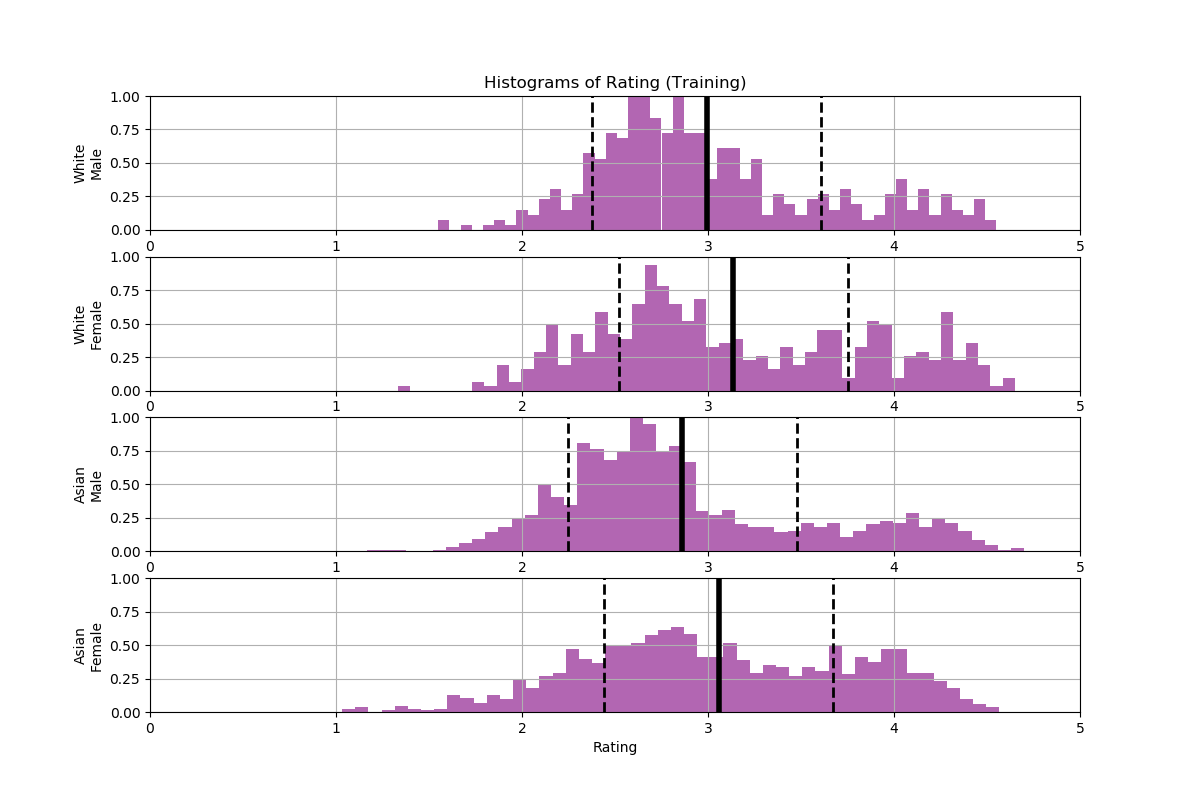
\includegraphics[width=.9\linewidth]{hist-train.png}
    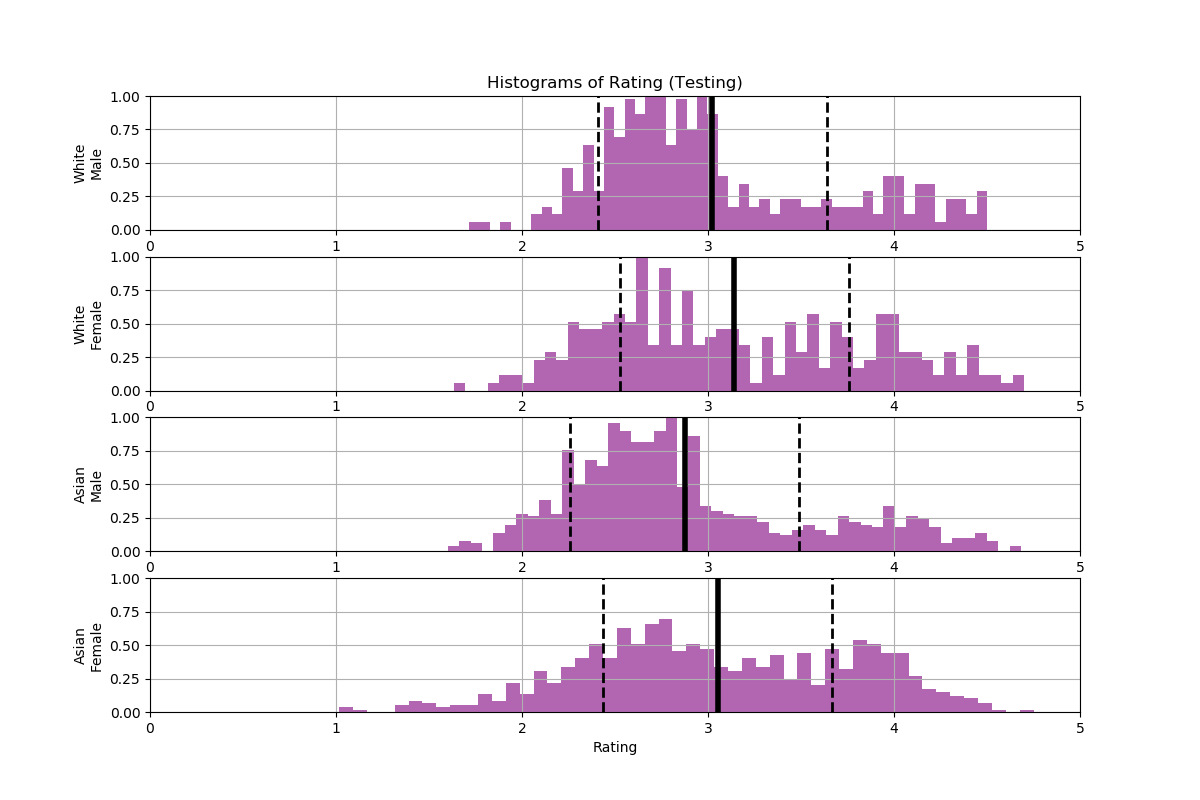
\includegraphics[width=.9\linewidth]{hist-test.png}
    \caption{Histograms of Scores}
    \label{histograms}
\end{figure}

Histogram visualizations showing the differences between each grouping is shown in Figure \ref{histograms}.  In these histograms we observe that the ratings do not follow a gaussian distribution.  Rather, most measurements are below the average and the mean is highly influenced by several high scoring outliers.  It is believed that the reason for this discrepancy comes from the fact that some of the images are from professional celebrity photoshoots, causing what appears to be a much smaller gaussian distribution at the high end of the ratings.

From this information we can gather it is likely that men's photos will be rated lower than women's on the trained model.  Furthermore, most photos will be considered below average.

\section{Design}

The Keras \citep{keras} machine learning framework was selected for implementation due to its ease of use and extremely high performance.  Keras implements its features with the TensorFlow \citep{tensorflow} machine learning framework, which is designed to take advantage of hardware numerical acceleration processors such as those included in the NVidia GPUs.

Following the neural network model architecture design of Shulga, a large network pre-trained to classify the ImageNet dataset was selected as the basis on which the face rating system was formed.  On top of the pre-trained network a tensor flatten layer was applied to reduce the dimensionality from 7$\times$7$\times$1024 to a single vector input of 50176.  This was fed into a 256 node fully-connected layer passed through a $tanh()$ activation funtion.  Finally a single node fully-connected layer was used to compute the output.  This differs somewhat from Shulga's design as he applied a single fully-connected layer for the output.

Shulga selected the ResNet50 \citep{resnet50} neural network architecture, however Keras includes several other pretrained networks.  A simple experiment was performed to determine which network would be the best for the task.

Each of the pre-trained networks in Keras was constructed as described above and tasked to train to perform a cat-vs-dog determination.  Accuracy and computational performance was measured and it was determined that MobileNet \citep{mobilenet}, not ResNet50 trained better but also consumed fewer resources.

The final neural network design is shown in Figure \ref{architecture}.

\newpage
\begin{figure}[H]
    \centering
    
\includegraphics[height=0.9\textheight]{architecture.png}
    \caption{Neural Network Architecture}
    \label{architecture}
\end{figure}

\subsection{Image Preprocessing}

Although the images are 350$\times$350 pixels in dimension, there is some inconsistency between images in the training set.  Some images have a white silhouette around the face while others do not.  Not all images were taken from the same distance, resulting in variation in the size of the faces.

A preprocessing step was performed to crop the image to 224$\times$224 pixels, the same size as the ImageNet inputs that the MobileNet was trained to.  First an OpenCV \citep{opencv} Haar feature-based cascade face classifier was used to identify faces within the scene.  The resulting bounding box around the face was cropped and rescaled to the desired 224$\times$224 image.

\begin{figure}[H]
    \centering
    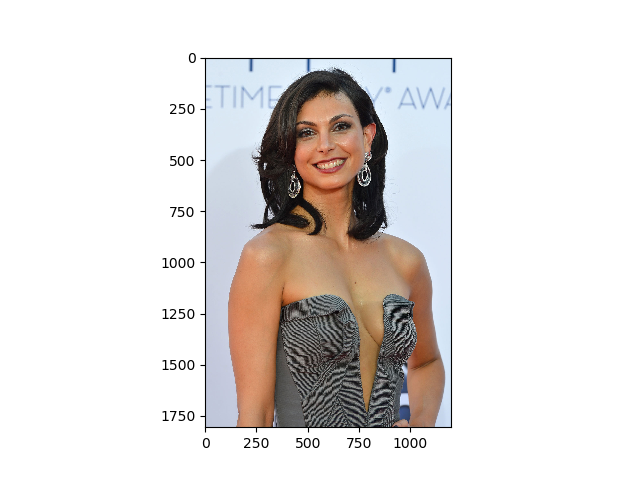
\includegraphics[width=.45\linewidth]{before-preprocessing.png}
    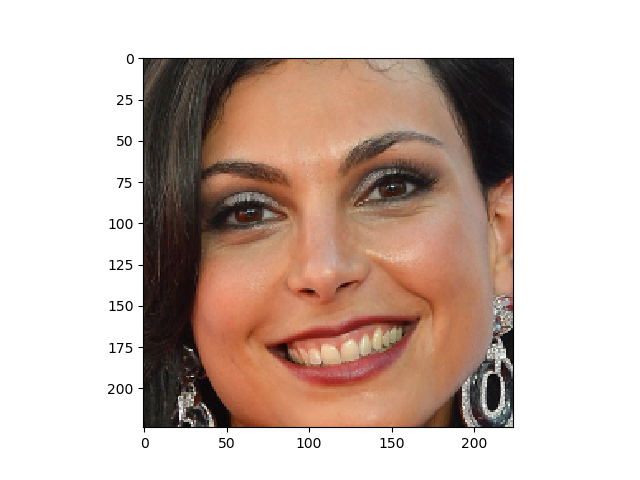
\includegraphics[width=.45\linewidth]{after-preprocessing.png}
    \caption{Before and After Preprocessing}
    \label{preprocessing}
\end{figure}

\subsection{Score Normalization}

Next the scores was adjusted from the 1-5 scale to a 1-10 scale, which is more commonly used in ratings from images to television shows and movies to interactions.  This was performed by subtracting the minimum value from the scores to set the lower bound to 0, then multiplying by 9 to create a 0-9 rating, and finally adding 1 to move the ratings to the 1-10 range.

This approach does not, however, redistribute the scores along a gaussian distribution.  In fact, the approach may bias scores lower towards the 1 rating.  Future work may revisit this technique to reduce the negative effects of receiving a lower than anticipated score on a personal photo.

\section{Training and Fine Tuning}

Training was performed in two stages:

\begin{enumerate}
    \item Training the new layers
    \item Fine-tuning the entire model
\end{enumerate}

To train the new layers, the MobileNet layer's trainable parameter was set to False.  During model compilation, Keras automatically constructs a neural network with fixed weights for these layers.

The input image dataset was augmented by performing random rotations on the input images of up to 30$^\circ$, shifting the input images in any direction up to 10\%, and performing up to 20\% rescaling of the images.  Keras provides this functionality automatically through the ImageDataGenerator object.

The training was performed over 30 epochs.  Training final statistics are in Figure \ref{training}.

\begin{table}[ht]
    \centering
    \begin{tabular}{|r|l|l|}
        \hline
        & Training & Validation \\ \hline
        Mean Square Error Loss & 0.8312 & 1.762 \\ \hline
        Mean Absolute Error & 0.7043 & 1.086 \\ \hline
    \end{tabular}
    \caption{Final Training Statistics}
    \label{training}
\end{table}

Fine-tuning was performed by recompiling the neural network model without setting any layer's training parameter to False.  Fine-tuning was then performed over 30 epochs.  Fine-tuning final statistics are shown in Figure \ref{fine-tuning}.

\begin{table}[ht]
    \centering
    \begin{tabular}{|r|l|l|}
        \hline
        & Training & Validation \\ \hline
        Mean Square Error Loss & 0.5088 & 0.5579 \\ \hline
        Mean Absolute Error & 0.6194 & 0.6061 \\ \hline
    \end{tabular}
    \caption{Final Training Statistics}
    \label{fine-tuning}
\end{table}

Of note is the radical improvement observed in the validation dataset in the fine-tuned values over the trained values.

TensorBoard visualization was performed of the training set to track these differences over time.  Visualization of the training is in Figure \ref{tensorboard-train} and visualization of the fine-tuning is in Figure \ref{tensorboard-fine-tune}.

\begin{figure}[H]
    \centering
    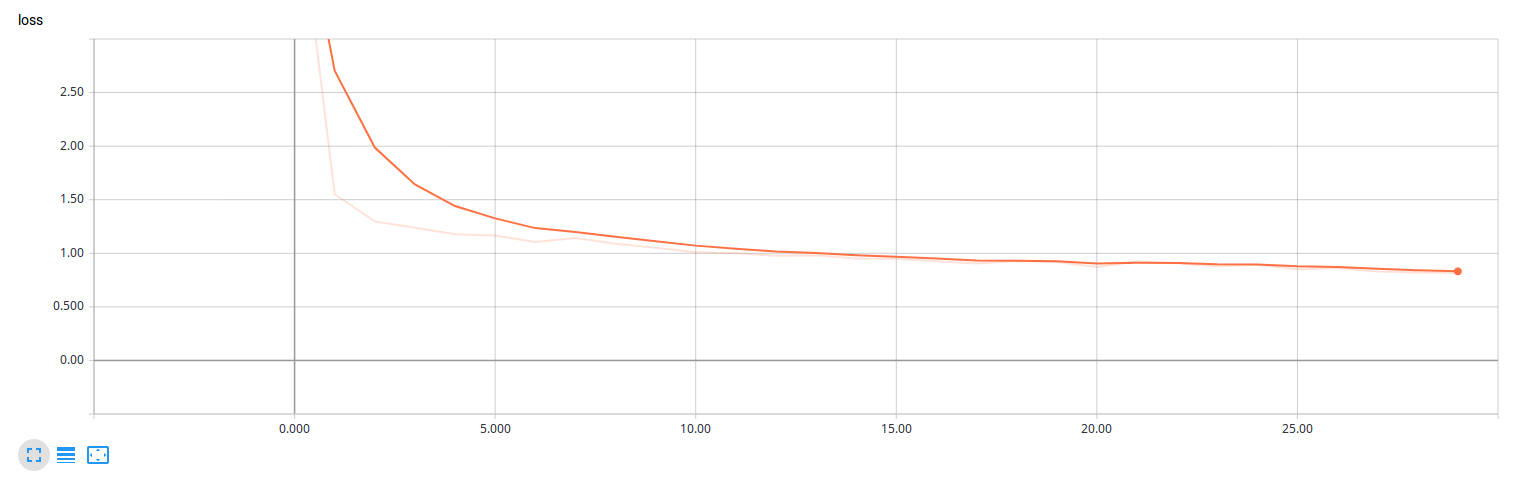
\includegraphics[width=.9\linewidth]{train-train-loss.png}
    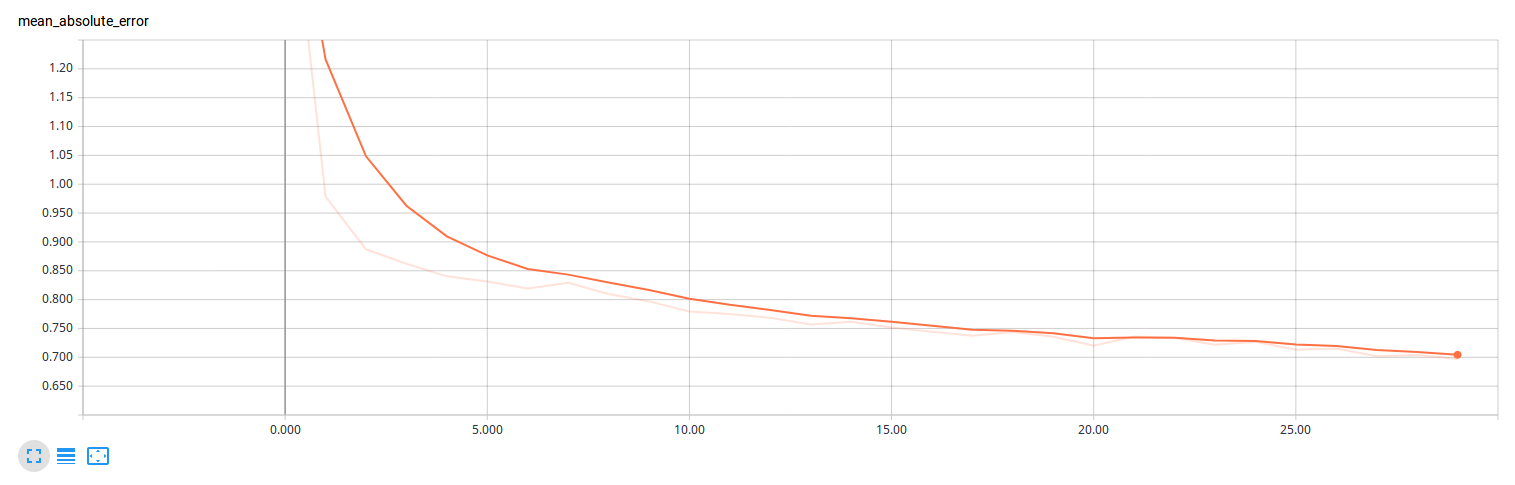
\includegraphics[width=.9\linewidth]{train-train-mean-abs-error.png}
    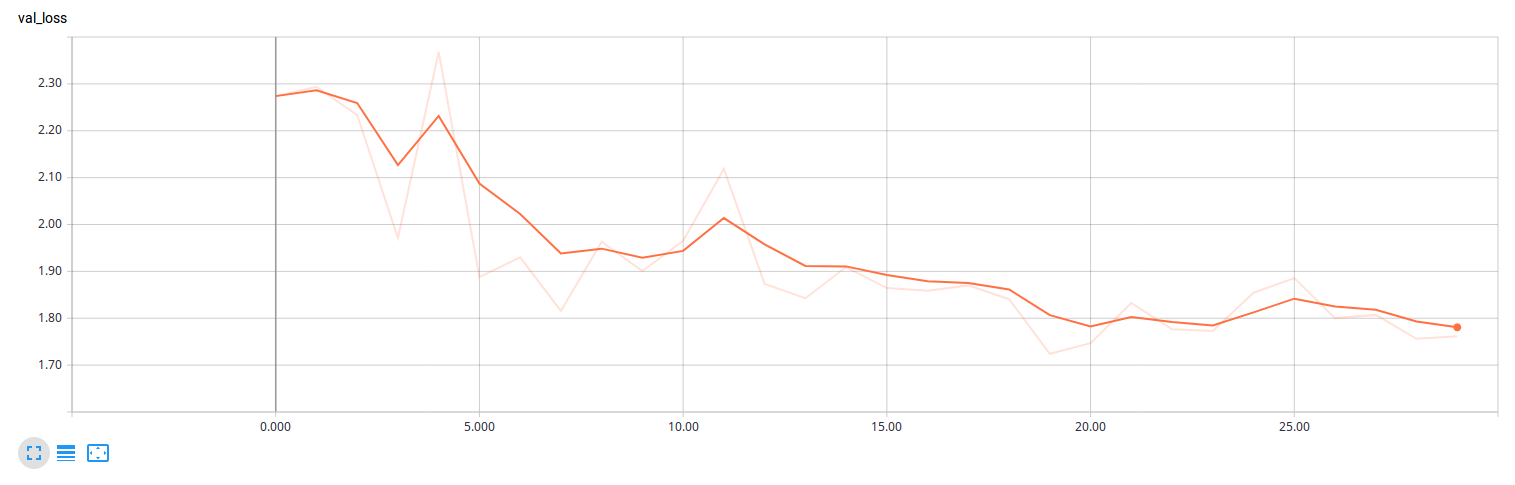
\includegraphics[width=.9\linewidth]{train-validation-loss.png}
    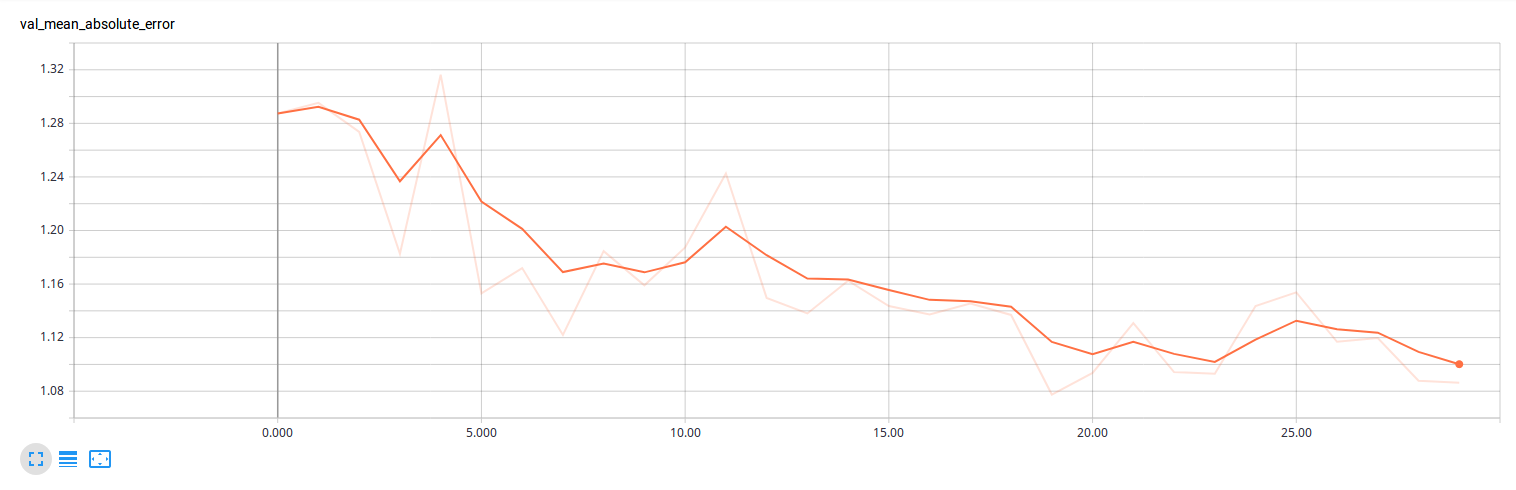
\includegraphics[width=.9\linewidth]{train-validation-mean-abs-error.png}
    \caption{Training Statistics}
    \label{tensorboard-train}
\end{figure}

\begin{figure}[H]
    \centering
    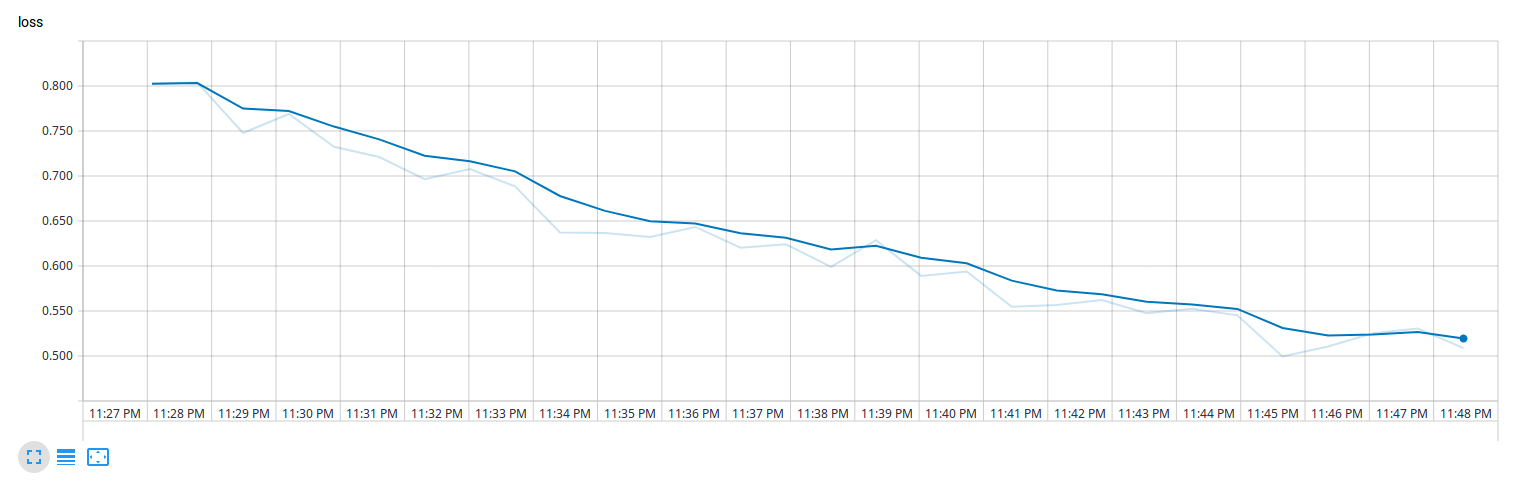
\includegraphics[width=.9\linewidth]{fine-tune-train-loss.png}
    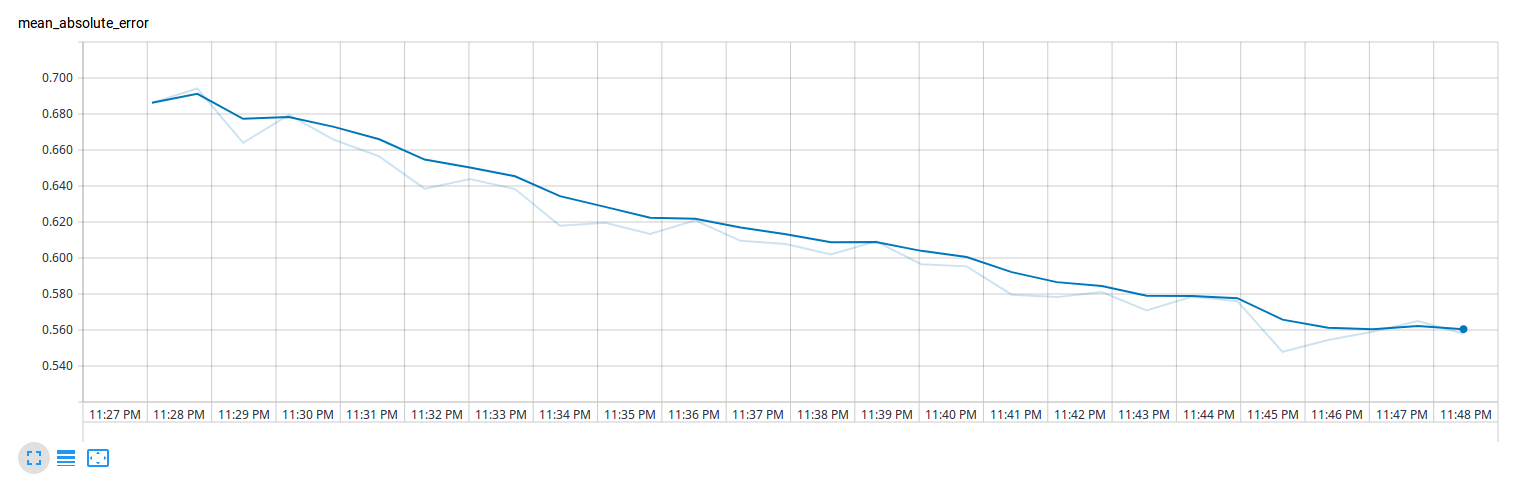
\includegraphics[width=.9\linewidth]{fine-tune-train-mean-abs-error.png}
    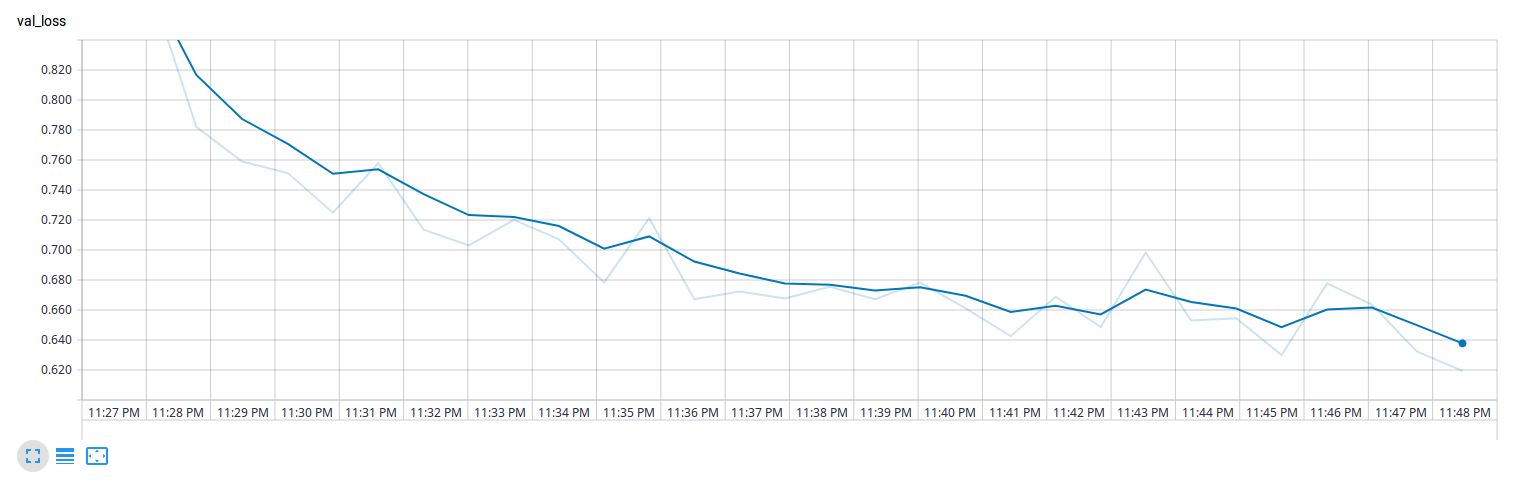
\includegraphics[width=.9\linewidth]{fine-tune-validation-loss.png}
    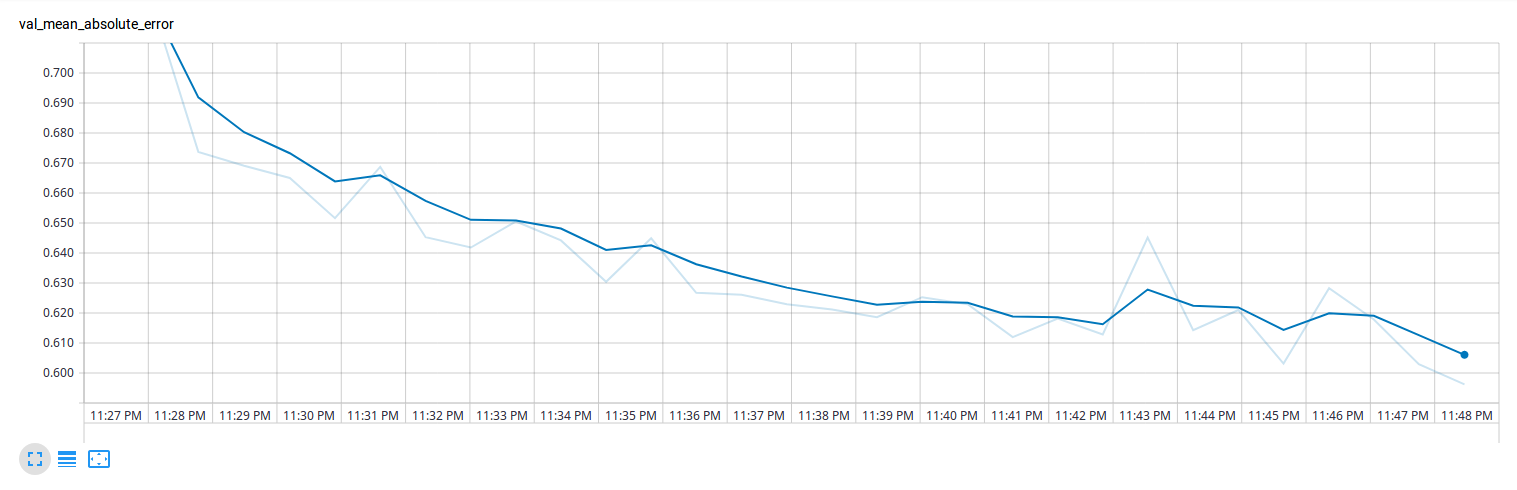
\includegraphics[width=.9\linewidth]{fine-tune-validation-mean-abs-error.png}
    \caption{Training Statistics}
    \label{tensorboard-fine-tune}
\end{figure}

The effects of fine-tuning are most profound when you examine the wall time graphs.  The mean square error loss and mean average error score of the training dataset follow a pseudo-linear trajectory, but the validation set shows a profound jump when transitioning from training to fine-tuning.  Visualization of the wall-time graphs is in Figure \ref{tensorboard-wall}.

\begin{figure}[H]
    \centering
    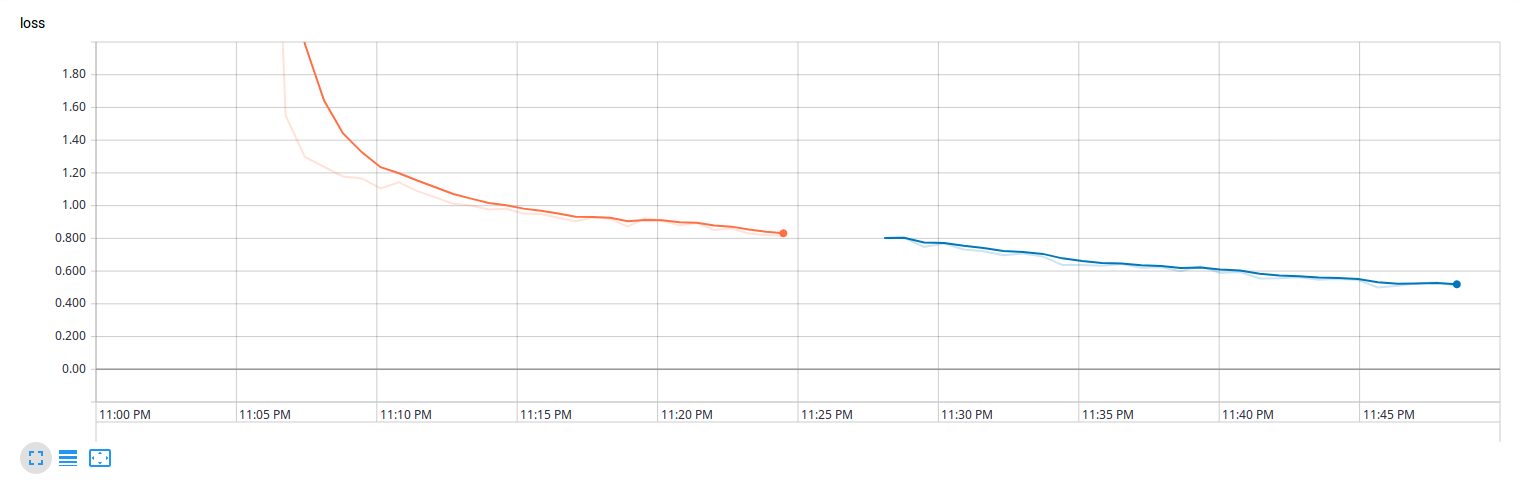
\includegraphics[width=.9\linewidth]{wall-train-loss.png}
    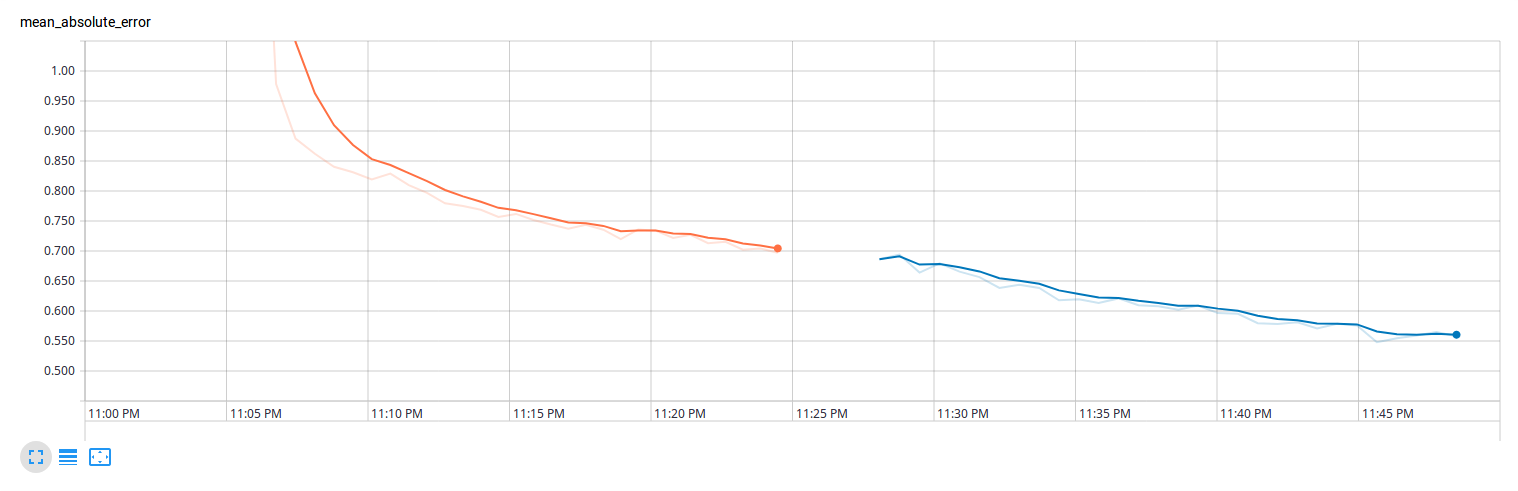
\includegraphics[width=.9\linewidth]{wall-train-mean-abs-error.png}
    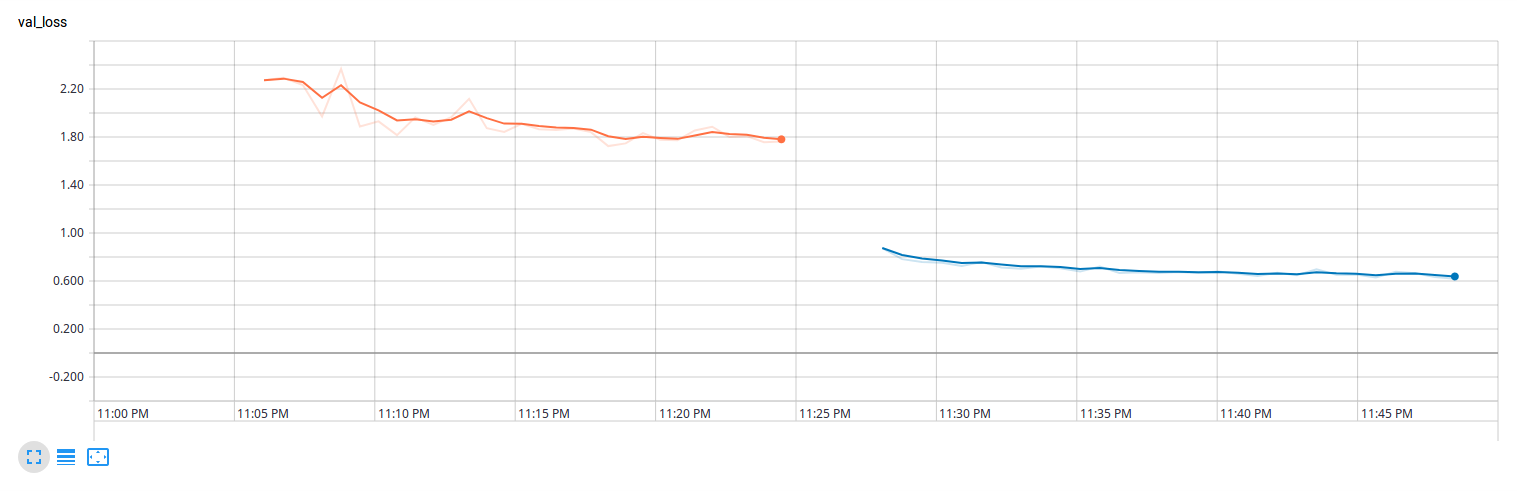
\includegraphics[width=.9\linewidth]{wall-validation-loss.png}
    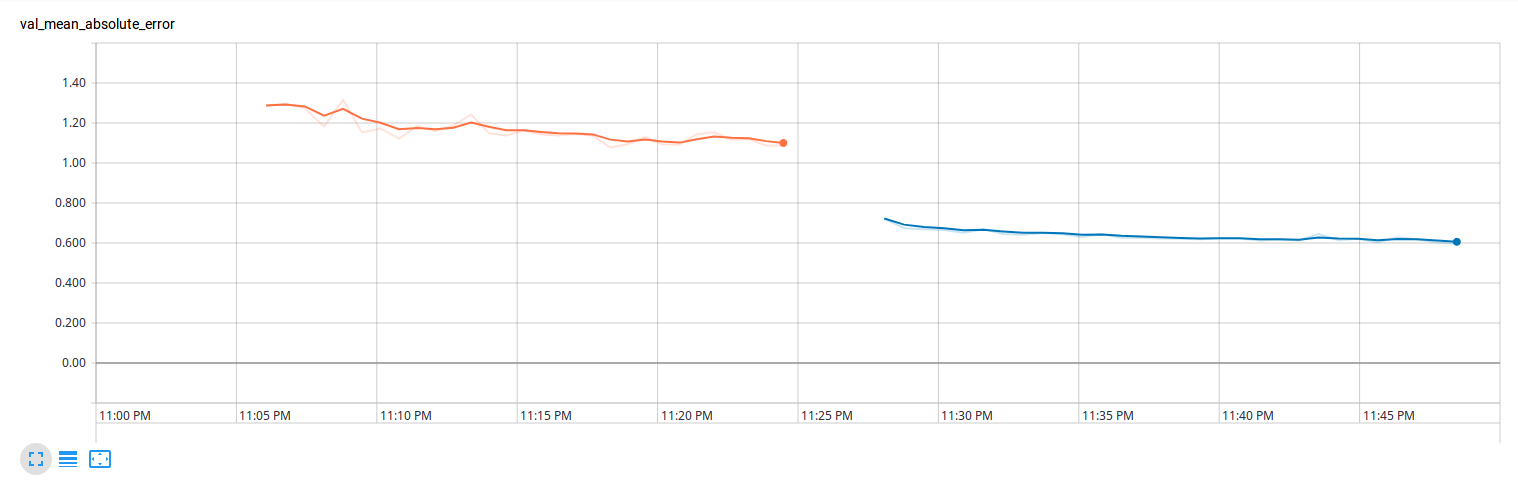
\includegraphics[width=.9\linewidth]{wall-validation-mean-abs-error.png}
    \caption{Training Statistics}
    \label{tensorboard-wall}
\end{figure}

\section{Testing}

Preprocessing of the images for testing purposes is identical to that of the training preprocessing.  OpenCV was again used for face detection, and each face was sent into the neural network to produce an output.

The images were then post-processed by adding rectangles around the detected faces and displaying the score values within the box.

\section{Results}

They also say a picture is worth a thousand words, so let's examine the results directly.

\begin{figure}[H]
    \centering
    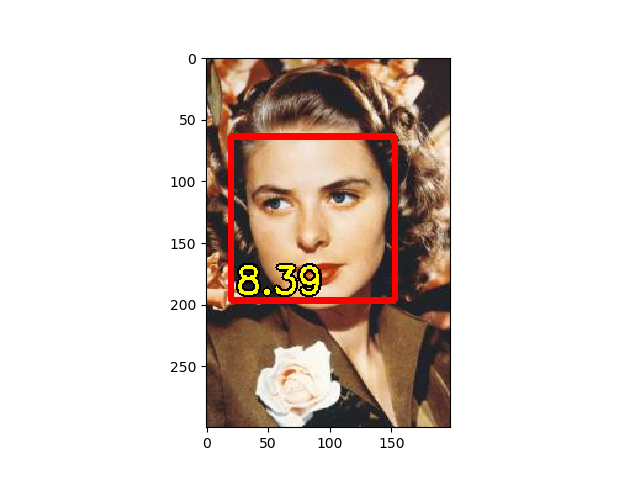
\includegraphics[width=.4\linewidth]{ingrid-bergman.png}
    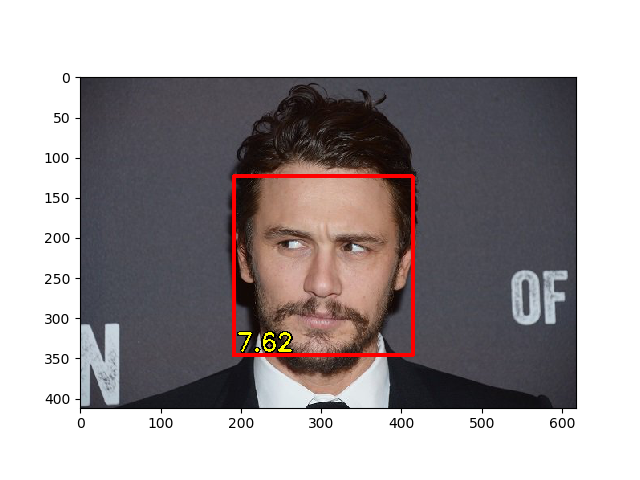
\includegraphics[width=.4\linewidth]{franco.png}
    \caption{Ingrid Bergman and James Franco}
\end{figure}

\begin{figure}[H]
    \centering
    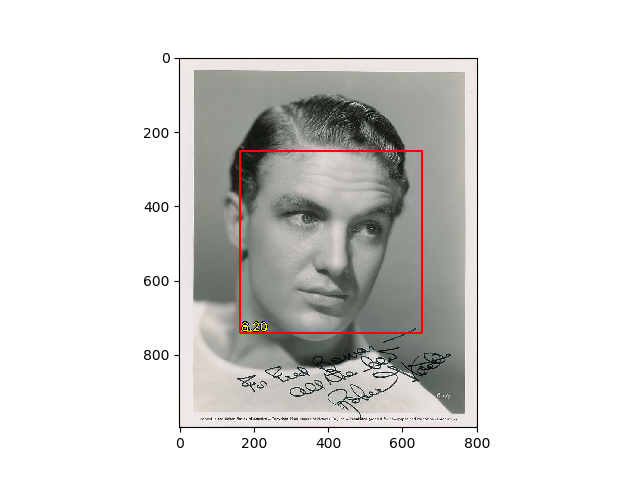
\includegraphics[width=.4\linewidth]{robert-stack-young.png}
    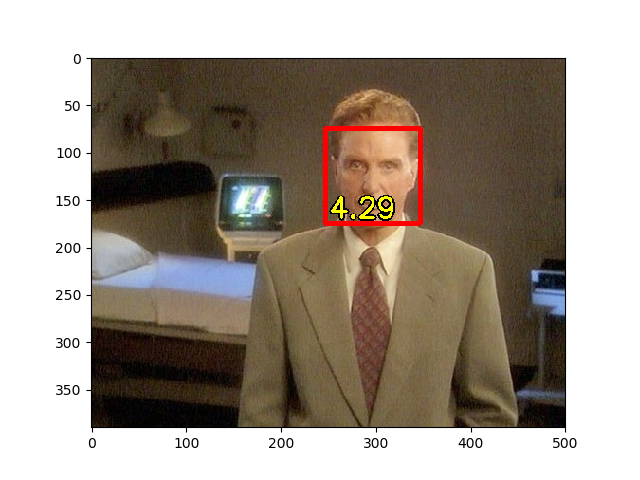
\includegraphics[width=.4\linewidth]{robert-stack-old.png}
    \caption{Robert Stack, Young and Old}
\end{figure}

\begin{figure}[H]
    \centering
    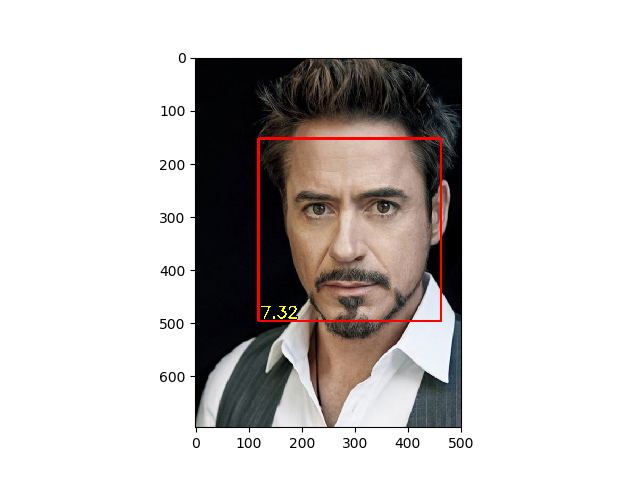
\includegraphics[width=.4\linewidth]{robert-downey-jr.png}
    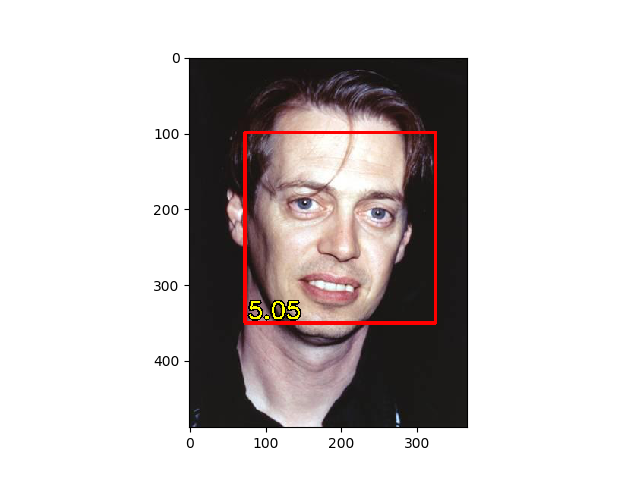
\includegraphics[width=.4\linewidth]{steve-buscemi.png}
    \caption{Robert Downey, Jr and Steve Buscemi}
\end{figure}

\begin{figure}[H]
    \centering
    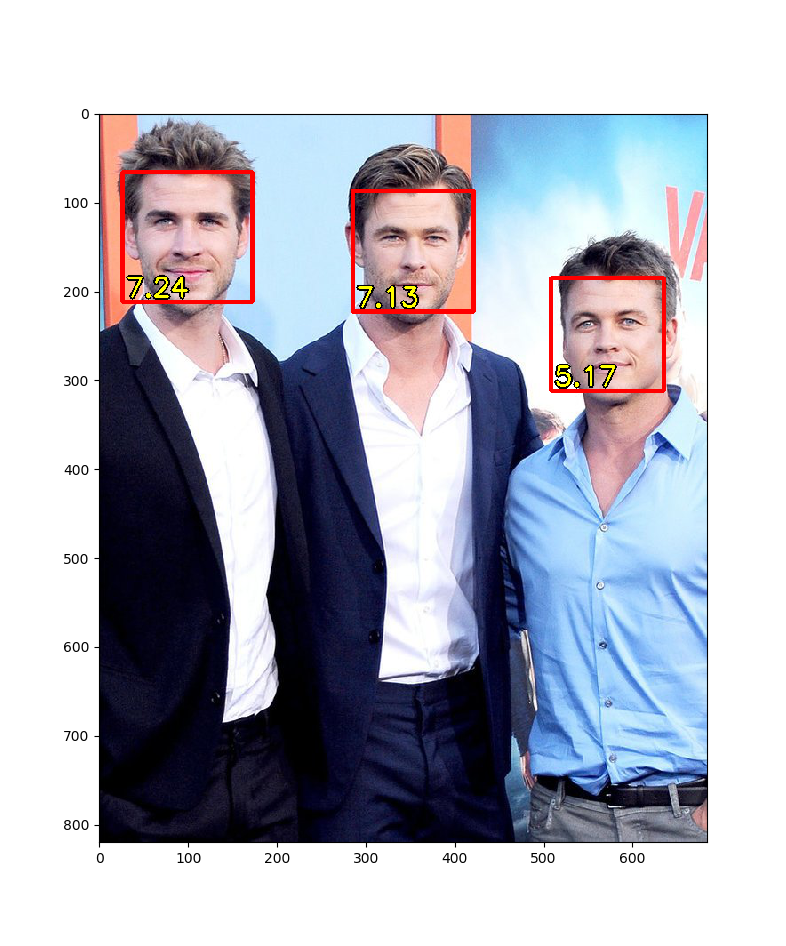
\includegraphics[width=.7\linewidth]{hemsworths.png}
    \caption{The Hemsworth Brothers}
\end{figure}

\begin{figure}[H]
    \centering
    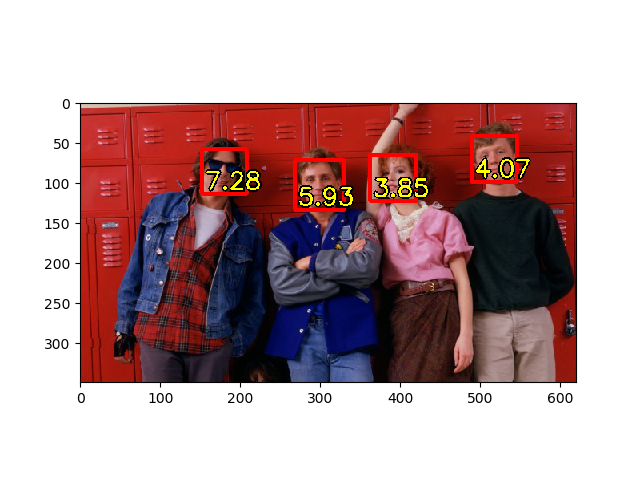
\includegraphics[width=.8\linewidth]{breakfast-club.png}
    \caption{The Breakfast Club}
\end{figure}

\begin{figure}[H]
    \centering
    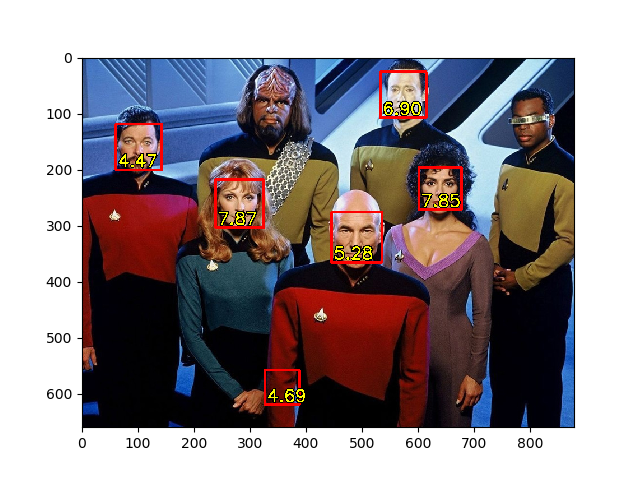
\includegraphics[width=.8\linewidth]{star-trek-tng.png}
    \caption{Star Trek: The Next Generation. Note: Geordi and Worf are not detected as faces by OpenCV, likely due the additional headgear.}
\end{figure}

\begin{figure}[H]
    \centering
    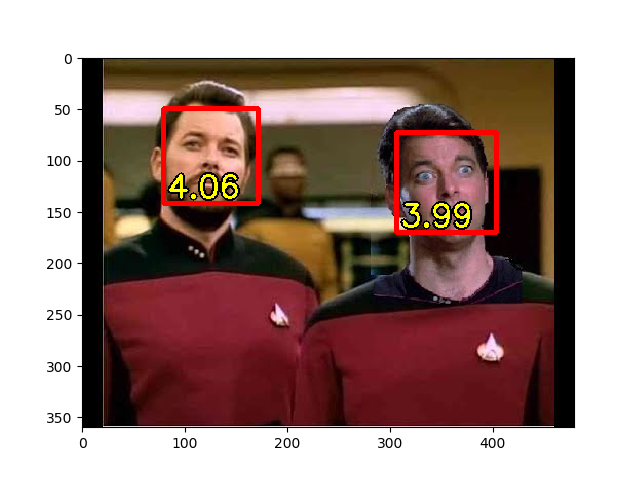
\includegraphics[width=.8\linewidth]{riker-beard.png}
    \caption{Beholder prefers Riker with a beard, as we all do!}
\end{figure}

\begin{figure}[H]
    \centering
    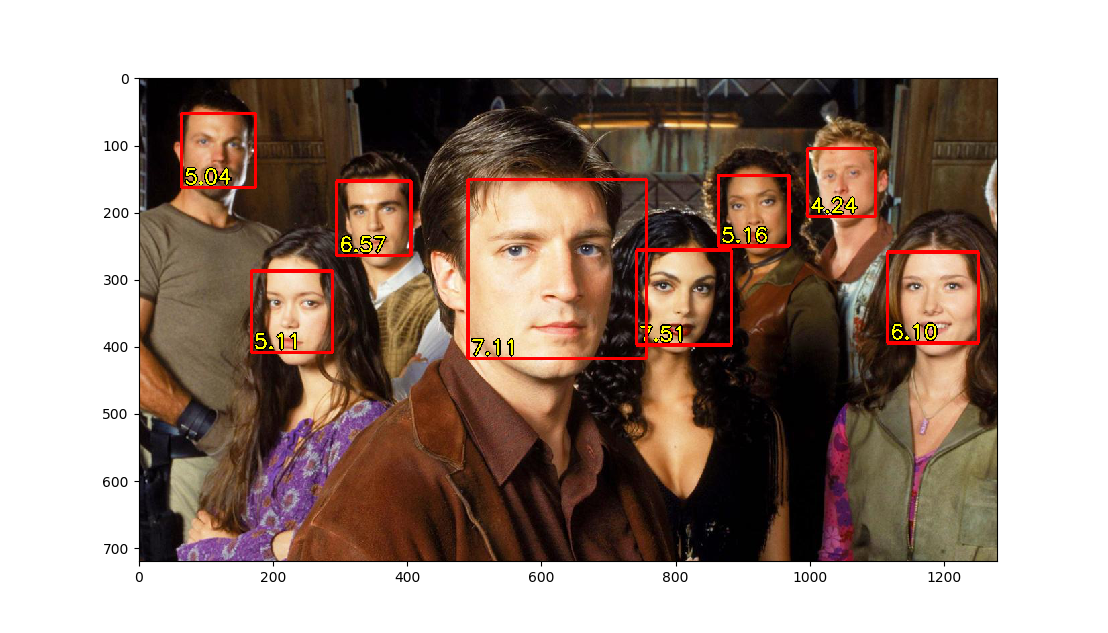
\includegraphics[width=.8\linewidth]{firefly.png}
    \caption{Firefly}
\end{figure}

\begin{figure}[H]
    \centering
    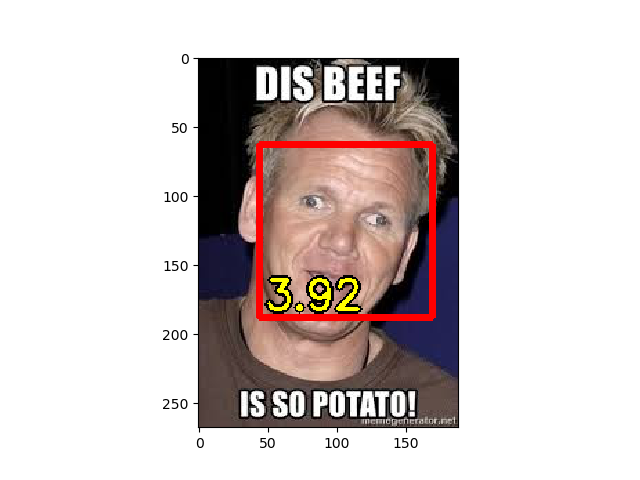
\includegraphics[width=.7\linewidth]{funny.png}
    \caption{A spicy meme a la Chef Ramsey}
\end{figure}

\begin{figure}[H]
    \centering
    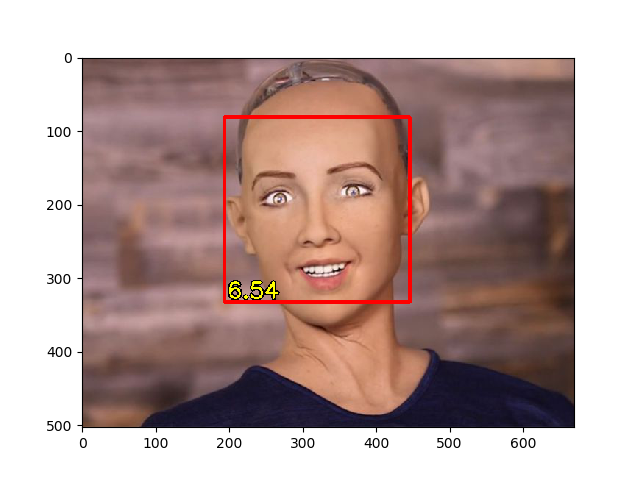
\includegraphics[width=.45\linewidth]{robot1.png}
    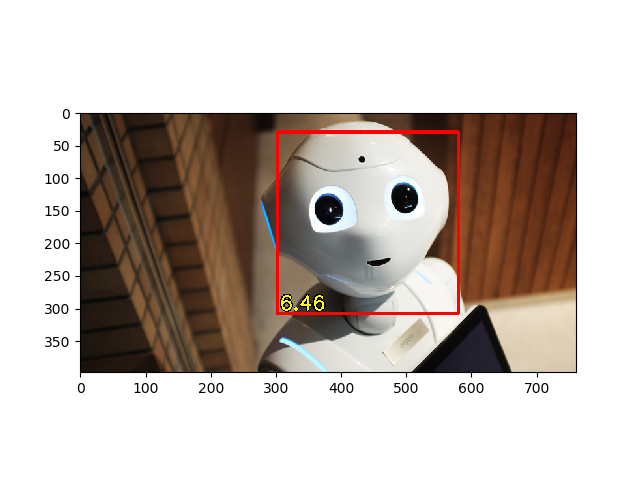
\includegraphics[width=.45\linewidth]{robot2.png}
    \caption{Even robots get rated!}
\end{figure}

\section{Conclusion and Future Work}

Using the Keras and TensorFlow frameworks along with the OpenCV library, it is a fairly straightforward process to construct a neural network to judge beauty in photos.  However, it should be noted that the neural network reflects the biases of the underlying data.  In this case it tends to rate average persons as below average, negatively penalizing men more than women.

If the values generated by the program are not taken as an actual 1-10 scoring, but as a relative metric, the the program may effectively be used to help winnow down the ideal photo for publication.

Possible future work could take place in constructing larger datasets with more ethnicities than White and Asian along with more age diversity than what was present in the SCUT5500-FBP dataset.  One approach would be to use metametrics such as social media connections, eliminating the need for manual scoring and permitting large scale dataset construction.  Another item worth looking into is forcing the scores to follow a gaussian distribution to remove some of the biases causing most images to show as low scoring.

Another avenue for exploration is to train a Generative Adversarial Network to the dataset allowing for one to input a photo, then adjust the score in latent space to generate images that may be more or less attractive than the original.

\medskip

\small

\bibliographystyle{te}
\bibliography{bibliography}

\end{document}
